% !TEX TS-program = XeLaTeX
% use the following command:
% all document files must be coded in UTF-8
\documentclass[portuguese]{textolivre}
% build HTML with: make4ht -e build.lua -c textolivre.cfg -x -u article "fn-in,svg,pic-align"

\journalname{Texto Livre}
\thevolume{16}
%\thenumber{1} % old template
\theyear{2023}
\receiveddate{\DTMdisplaydate{2023}{5}{7}{-1}} % YYYY MM DD
\accepteddate{\DTMdisplaydate{2023}{6}{26}{-1}}
\publisheddate{\DTMdisplaydate{2023}{8}{14}{-1}}
\corrauthor{Fernando da Costa Barbosa}
\articledoi{10.1590/1983-3652.2023.46113}
%\articleid{NNNN} % if the article ID is not the last 5 numbers of its DOI, provide it using \articleid{} commmand 
% list of available sesscions in the journal: articles, dossier, reports, essays, reviews, interviews, editorial
\articlesessionname{articles}
\runningauthor{Barbosa et al.} 
%\editorname{Leonardo Araújo} % old template
\sectioneditorname{Daniervelin Pereira}
\layouteditorname{Deive Barbosa Alves}

\title{O Automated Guided Vehicle como um micromundo de aprendizagem matemática: uma perspectiva construcionista}
\othertitle{The Automated Guided Vehicle as a mathematical learning microworld: a constructionist perspective}
% if there is a third language title, add here:
%\othertitle{Artikelvorlage zur Einreichung beim Texto Livre Journal}

\author[1]{Fernando da Costa Barbosa~\orcid{0000-0001-8558-3521}\thanks{Email: \href{mailto:fcbarbosa@ufcat.edu.br}{fcbarbosa@ufcat.edu.br}}}
\author[1]{Daniel da Silveira Guimarães~\orcid{0000-0003-1973-9609}\thanks{Email: \href{mailto:danielguimaraes@ufg.br}{danielguimaraes@ufg.br}}}
\author[1]{Élida Alves da Silva~\orcid{0000-0001-5417-9083}\thanks{Email: \href{mailto:elida\_alves@ufg.br}{elida\_alves@ufg.br}}}
\author[2]{Deive Barbosa Alves~\orcid{0000-0002-0850-7362}\thanks{Email: \href{mailto:deivealves@ufnt.edu.br}{deivealves@ufnt.edu.br}}}
\author[3]{Mônica da Cunha Alves~\orcid{0009-0004-0780-5706}\thanks{Email: \href{mailto:monicaefauez@gmail.com}{monicaefauez@gmail.com}}}

\affil[1]{Universidade Federal de Catalão, Catalão, GO, Brasil.}
\affil[2]{Universidade Federal do Tocantins, Palmas, TO, Brasil}
\affil[3]{Colégio Estadual João Bernardes de Assunção, Davinópolis, GO, Brasil.}

\addbibresource{article.bib}
% use biber instead of bibtex
% $ biber article

% used to create dummy text for the template file
\definecolor{dark-gray}{gray}{0.35} % color used to display dummy texts
\usepackage{lipsum}
\SetLipsumParListSurrounders{\colorlet{oldcolor}{.}\color{dark-gray}}{\color{oldcolor}}

% used here only to provide the XeLaTeX and BibTeX logos
\usepackage{hologo}

% if you use multirows in a table, include the multirow package
\usepackage{multirow}

% provides sidewaysfigure environment
\usepackage{rotating}

% CUSTOM EPIGRAPH - BEGIN 
%%% https://tex.stackexchange.com/questions/193178/specific-epigraph-style
\usepackage{epigraph}
\renewcommand\textflush{flushright}
\makeatletter
\newlength\epitextskip
\pretocmd{\@epitext}{\em}{}{}
\apptocmd{\@epitext}{\em}{}{}
\patchcmd{\epigraph}{\@epitext{#1}\\}{\@epitext{#1}\\[\epitextskip]}{}{}
\makeatother
\setlength\epigraphrule{0pt}
\setlength\epitextskip{0.5ex}
\setlength\epigraphwidth{.7\textwidth}
% CUSTOM EPIGRAPH - END

% LANGUAGE - BEGIN
% ARABIC
% for languages that use special fonts, you must provide the typeface that will be used
% \setotherlanguage{arabic}
% \newfontfamily\arabicfont[Script=Arabic]{Amiri}
% \newfontfamily\arabicfontsf[Script=Arabic]{Amiri}
% \newfontfamily\arabicfonttt[Script=Arabic]{Amiri}
%
% in the article, to add arabic text use: \textlang{arabic}{ ... }
%
% RUSSIAN
% for russian text we also need to define fonts with support for Cyrillic script
% \usepackage{fontspec}
% \setotherlanguage{russian}
% \newfontfamily\cyrillicfont{Times New Roman}
% \newfontfamily\cyrillicfontsf{Times New Roman}[Script=Cyrillic]
% \newfontfamily\cyrillicfonttt{Times New Roman}[Script=Cyrillic]
%
% in the text use \begin{russian} ... \end{russian}
% LANGUAGE - END

% EMOJIS - BEGIN
% to use emoticons in your manuscript
% https://stackoverflow.com/questions/190145/how-to-insert-emoticons-in-latex/57076064
% using font Symbola, which has full support
% the font may be downloaded at:
% https://dn-works.com/ufas/
% add to preamble:
% \newfontfamily\Symbola{Symbola}
% in the text use:
% {\Symbola }
% EMOJIS - END

% LABEL REFERENCE TO DESCRIPTIVE LIST - BEGIN
% reference itens in a descriptive list using their labels instead of numbers
% insert the code below in the preambule:
%\makeatletter
%\let\orgdescriptionlabel\descriptionlabel
%\renewcommand*{\descriptionlabel}[1]{%
%  \let\orglabel\label
%  \let\label\@gobble
%  \phantomsection
%  \edef\@currentlabel{#1\unskip}%
%  \let\label\orglabel
%  \orgdescriptionlabel{#1}%
%}
%\makeatother
%
% in your document, use as illustraded here:
%\begin{description}
%  \item[first\label{itm1}] this is only an example;
%  % ...  add more items
%\end{description}
% LABEL REFERENCE TO DESCRIPTIVE LIST - END


% add line numbers for submission
%\usepackage{lineno}
%\linenumbers

\begin{document}
\maketitle

\begin{polyabstract}
\begin{abstract}
O artigo buscou explorar, em uma perspectiva construcionista, o Automated Guided Vehicle (AGV) enquanto um Micromundo de aprendizagem matemática. A sua constituição se deu a partir de uma pesquisa qualitativa do tipo exploratória, ou seja, aquela em que se deseja oferecer uma visão geral sobre o objeto. Nesse processo, foram realizadas pesquisas bibliográficas, baseadas em estudos de autores como, por exemplo, Seymour Papert, Pierre Lèvy, e marcada pela experimentação baseada em \textcite{Guimaraes2020}. Assim, estabeleceu-se como objetivo estudar a viabilidade de adotar o AGV como micromundo de aprendizagem matemática, na perspectiva da bricolagem, simulação e inteligência criadora. A experiência com a construção do AGV é mais que a construção de um robô, é a afirmação da importância da Matemática, do simulador virtual na concepção do real, do tangível.

\keywords{Inteligência criadora \sep Robótica educacional \sep Micromundo \sep Aprendizagem matemática}
\end{abstract}

\begin{english}
\begin{abstract}
The article sought to explore, from a constructionist perspective, the Automated Guided Vehicle (AGV) as a Microworld for mathematical learning. Its constitution took place from qualitative exploratory research, in which an overview of the object is offered. In this process, bibliographical research was conducted, based on studies by authors such as Seymour Papert, Pierre Lèvy and marked by experimentation based on \textcite{Guimaraes2020}. Thus, the objective was to study the feasibility of adopting AGV as a Microworld for mathematical learning, from the perspective of bricolage, simulation, and creative intelligence. The experience with the construction of AGV is more than the construction of a robot, it is the affirmation of the importance of Mathematics, virtual simulation in the conception of the real, and the tangible.

\keywords{Creative intelligence \sep Educational robotics \sep Microworld \sep Mathematical learning}
\end{abstract}
\end{english}
% if there is another abstract, insert it here using the same scheme

\end{polyabstract}

\section{Introdução}\label{sec-intro}
As tecnologias digitais vêm transformando a vida das pessoas e a realidade do mercado de trabalho de forma muito dinâmica, em que é o caso da Robótica Educacional. É papel das instituições de ensino preparar as crianças e jovens de forma que sejam capazes de se adaptarem a essa realidade. Segundo \textcite[p. 27]{SantosPaulo2019}, “[...] a educação deve se incumbir da tarefa de se apropriar da agenda tecnológica do nosso tempo, da nossa época tecnológica, com suas particularidades e contradições”. Contudo, para muitos estudantes, especialmente da rede pública de ensino, a robótica não faz parte do cotidiano. Neste sentido, é necessário que as referidas instituições sejam (re)pensadas e (re)desenhadas para atender as demandas postas.

Sabe-se que os recursos destinados às instituições de ensino públicas não são suficientes para proporcionar a implementação do ensino de robótica a partir de kits proprietários. Porém, os estudantes não podem ser privados do desenvolvimento de habilidades e competências que possibilitem sua adaptação à nova realidade. \textcite[p. 2]{Guimaraes2020} afirmam que “[...] inserir uma robótica educacional com baixo custo em escolas públicas do país, é oportunizar acesso à uma educação tecnológica para indivíduos que não usufruem dela nos moldes operantes no país”. Ou seja, pressupõem trabalhar com a Robótica Educacional Livre (REL), que propicia a popularização da robótica, e que converge com a concepção defendida por \textcite[p. 4]{CesarDanilo2009} “[...] a utilização de uma práxis pautada na liberdade vem da crença de que o conhecimento produzido pela humanidade deve ser compartilhado por todos, sem que seja visto como propriedade particular”.

Na expectativa de contribuir com a difusão de conhecimentos propiciados pela REL, propôs-se a criação de um Micromundo a partir da construção de um veículo auto guiado, em inglês \emph{Automated Guided Vehicle} (AGV), que segue uma linha a custo zero. Em \textcite{Guimaraes2020} foi feita uma exploração desse Micromundo, onde se propôs diversas atividades para o processo de ensino e aprendizagem de Matemática a partir de um robô seguidor de linha, feito totalmente com materiais advindos da sucata de equipamentos tecnológicos. Para a validação da proposta, foi realizada uma investigação na qual os participantes envolvidos criaram dois protótipos de AGV, um simulado e um real, e os compatibilizaram a partir de parâmetros matemáticos. Este artigo traz, portanto, reflexões sobre o processo de ensino e aprendizagem desenvolvido neste Micromundo sob uma perspectiva constituída a partir de três elementos: a bricolagem, a simulação de modelos digitais e a inteligência criadora.


\section{Fundamentação teórica}\label{sec-normas}
Este artigo buscou explorar, em uma perspectiva construcionista, o \emph{Automated Guided Vehicle} (AGV) enquanto um Micromundo de aprendizagem matemática. O objetivo nesta seção é, então, esclarecer nosso entendimento sobre: o Construcionismo, Micromundo e os estilos de aprendizagem construcionistas.

Existem dois polos antagônicos nos modos de ensino da Educação: o Instrucionismo e o Construcionismo. A diferença entre os dois polos é bastante clara. Os instrucionistas acreditam que a aprendizagem é o resultado direto do ensino, buscando reformar a educação por meio de livros didáticos, testes e mudanças na prática docente. No entanto, os construcionistas sustentam que a aprendizagem resulta da experiência e que a compreensão é construída dentro da cabeça do aprendiz em um contexto social. Os professores construcionistas procuram criar experiências que valorizem o conhecimento dos alunos e os exponham a ideias inspiradoras. Os autores afirmam que o ensino instrucionista só é adequado quando a instrução é útil para aprender coisas rápidas ou de pouco benefício em investigá-las, enquanto a aprendizagem é mais efetiva quando está integrada a atividades que envolvem a construção de um produto significativo \cite{Papert1986, Martinez2019}.

A experiência que o contexto construcionismo advoga se refere ao conhecimento que se aprende investigando experimentos. E o ambiente do mundo real controlado para o estudante explorar, descobrir e simular acontecimentos,\textcite[p. 151]{Papert1985} chamou de Micromundo, o qual ele conceitua como “[...] um ambiente de aprendizagem interativo que tem como base o computador, em que os pré-requisitos estão embutidos no sistema e em que os aprendizes podem tornar-se ativos arquitetos construtores de sua própria aprendizagem”.

O veículo auto guiado, AGV, é nosso Micromundo, o qual possibilitou que os sujeitos pesquisados assumissem dois papéis nas formas de organizar, conhecer e pensar, tanto os elementos básicos da computação quanto aprender matemática. Houve momentos que eles assumiram o papel do “Planejador” e, em outros, o papel de \emph{“Bricoleur”}.

Para \textcite[p. 6]{Papert1992} os “[..]\emph{Bricoleurs} constroem teorias arranjando e reorganizando, negociando e renegociando com um conjunto de materiais conhecidos”. Ele faz as coisas do jeito dele. Quem assume esse papel resiste à ideia de que o geral é superior ao específico ou que abstrato é superior ao concreto, o produto emerge por meio de uma negociação entre ele e seu material. “[...] na culinária, esse seria o estilo dos chefs que não seguem receitas, mas uma série de decisões tomadas em função do sabor das coisas” \cite[p. 7]{Papert1992}. Para o \emph{Bricoleur}, o caminho para aquisição de um conhecimento técnico não passa por um projeto estrutural, mas pelo prazer de deixar os efeitos emergirem.

Na outra ponta estão os Planejadores que se diferenciam dos \emph{Bricoleurs}, não na qualidade do produto, mas no processo de criá-lo. Para eles, o modo de produção começa com um plano claro e definido em termos abstratos, produzindo parte por parte e só no final as une para ter um produto na versão final. O estilo de produção dos Planejadores são as formas culturais predominantes nos espaços escolares, considerada a maneira de pensar canônica a ser ensinada \cite{Papert1992}.

Os estilos Planejadores e \emph{Bricoleurs} produzem jeitos de pensar diferentes, no processo de criação e construção de conhecimento. Esses autores permitem a interpretação que tais estilos são inconciliáveis, uma vez que estudantes \emph{Bricoleurs} “[...] negam quem são para ter sucesso” \cite[p. 3]{Papert1992}. Contudo o trabalho de Marina \citeyear{Marina2009} busca conciliar esses dois mundos no que ele chamou de Inteligência Criadora. Em outras palavras, tanto \textcite{Papert1992} quanto \textcite{Marina2009} partem da pluralidade de formas de invenção de si e do mundo, sejam os primeiros pelo estilo de produzirem ciência e tecnologia ou o segundo pela diversidade de inteligência que nos permite conhecer a realidade. Entre essa diversidade \textcite[p. 6-9]{Marina2009} teoriza sobre a Inteligência Criadora, compreendida como “[...] aptidão para organizar comportamentos, descobrir valores, inventar e sustentar projetos, ser capaz de se libertar do determinismo da situação, resolver problemas, saber colocá-los”, é ela que “nos permite conhecer a realidade”. Criadora porque o humano tem uma inquietação, “[...] que transforma a humanidade em um fornecedor permanente de novidades ambivalentes [...]”, que inventa possibilidades na realidade. “[...] as coisas têm propriedades reais, nas quais inventamos possibilidades livres. Na propriedade real do petróleo, que é produzir energia, o homem descobriu a possibilidade de voar. [...] Inventamos verdades. Damos às coisas possibilidade de confirmar uma verdade científica” \cite [p. 10-11]{Marina2009}.

Se no construcionismo papertiano temos os Micromundos, na Teoria da Inteligência Criadora tem-se o projeto, ambiente de aprendizagem que de “[...] irrealidade em irrealidade, chegamos à realidade, depois de percorrer um longo itinerário de ideias, esboços, desenhos, comparações, planos, [...], maldições e aplausos”. O projeto como irrealidade “[...] é uma informação que pode ser atualizada, elaborada e atualizada fora de contexto, em estado livre ou isento” \cite[p. 205]{Marina2009}. No escopo deste trabalho se tem o projeto de um robô seguidor de linha, o projeto AGV, para ensinar matemática.

Se no estilo \emph{Bricoleurs} observa-se a busca de um caminho próprio com a metáfora da culinária: “[...] na culinária, esse seria o estilo dos chefs que não seguem receitas, mas uma série de decisões tomadas em função do sabor das coisas” \cite[p. 7]{Papert1992}. De acordo com \textcite[p.163]{Marina2009} vê-se a mesma subjetividade criadora, pois o “[...] criador seleciona sua própria informação, comanda sua visão sobre a realidade e estabelece suas próprias metas”. Evitando recorrer aos cânones vigentes, pois ao fazê-lo “[...] estará enclausurando na repetição”.

A subjetividade criadora em \textcite{Marina2009} comunga da característica do estilo Planejador, de \textcite{Papert1992}, pois o todo criado, o AGV, já é um projeto. Projetos como ideia, irrealidade no sentido de estrutura pensada para produzir algo, ou melhor, “[...] possibilidade escolhida, aquela que está ordenada à “realização”. [...] Depois que se entrega o controle ao projeto, ele reorganiza todo o comportamento.” \cite[p. 117]{Marina2009}. Mas esse autor também dá características do estilo \emph{Bricoleurs} ao projeto quando ele cria à concepção de projeto criador, o qual

\begin{quote}
[...] é uma invenção do indivíduo, está ao mesmo tempo dentro e fora dele – poderíamos considerá-lo como uma ampliação ou prolongamento dele -, mas este “fora” pode ser mais ou menos próximo, mais ou menos previsível. [...] Quando formulamos um projeto inventivo, localizamos a meta num lugar problemático e distante, para o qual somos atraídos. [...] Estamos falando de atividades recorrentes que podem andar em círculos sobre si mesmas. \cite[p. 119]{Marina2009}.
\end{quote}

Outro dizer corrobora com o referido entrelaçamento, em que: “[...] o projeto começa como um assunto indigente de busca, talvez suscitado pelo acaso, mas é preciso explicar por quais enigmáticas influências este começo pobre chega a dirigir, animar e controlar a ação criadora” \cite[p. 122]{Marina2009}. Conforme mencionado previamente, a ação criativa do projeto AGV se dividiu em dois projetos distintos: o protótipo AGV simulado em computador e o protótipo AGV físico construído a partir da reciclagem de componentes eletrônicos. Essas duas abordagens serão exploradas em seções subsequentes.


\section{Metodologia}\label{sec-modelo}
O artigo parte de uma pesquisa qualitativa do tipo exploratória, ou seja, aquela em que se deseja oferecer uma visão geral sobre o objeto, principalmente quando “[...] o tema escolhido é pouco explorado e torna-se difícil sobre ele formular hipóteses precisas e operacionalizáveis” \cite[p. 27]{GilAntonio2008}. A pesquisa foi também pautada em pesquisas bibliográficas, baseada em estudos de autores, como por exemplo Papert, Marina, Lèvy e Nunes, entre outros, e marcada pela experimentação baseada em \textcite{Guimaraes2020}. O artigo buscou responder, desta forma, a seguinte inquietação: como podemos desenvolver um trabalho de inteligência criadora com REL e Matemática? Neste sentido, estabeleceu-se como objetivo estudar a viabilidade de adotar o AGV como Micromundo de ensino e aprendizagem da Matemática, na perspectiva da bricolagem, simulação e inteligência criadora. 

O AGV é um carrinho, construído a partir de materiais recicláveis, na concepção proposta pela robótica livre, que deve “[...] percorrer uma trajetória, construída com linha preta em uma superfície clara, com velocidade e tempo gasto otimizados” \cite[p. 5]{Guimaraes2020}, como podemos ver na \Cref{figura01} seu modelo real (protótipo).

\begin{figure}[htbp]
\centering
\begin{minipage}{.8\textwidth}
 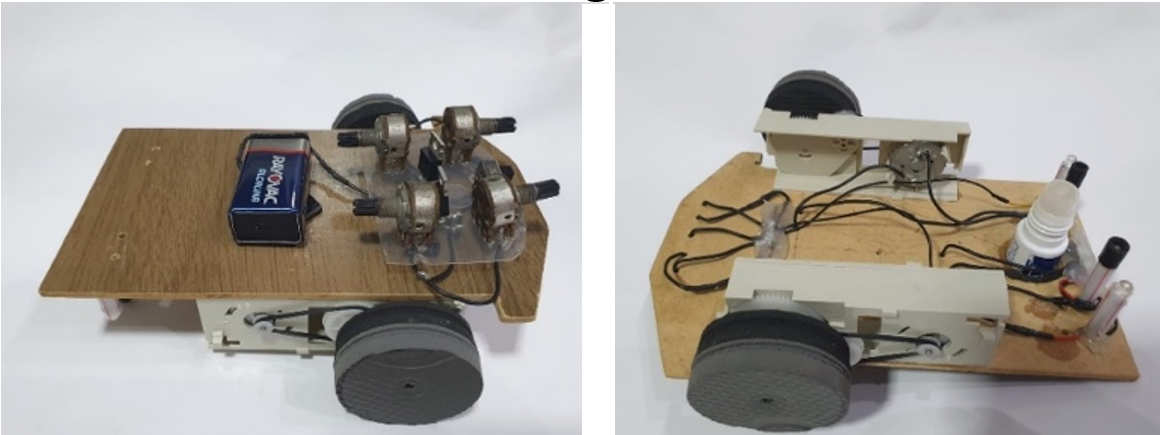
\includegraphics[width=\textwidth]{figuras/figura 1.png} 
 \caption{AGV:}
 \label{figura01}
 \source{Alves \citeyear[p. 48]{AlvesMonica2022}.}
\end{minipage}
\end{figure}

O modelo real se traduz na abstração, do desenho técnico eletrônico, apresentado na \Cref{figura02}, onde podemos observar: os componentes eletrônicos, os motores, os sensores, a fonte de alimentação de nove volts e os seus circuitos formados.

\begin{figure}[htbp]
\centering
\begin{minipage}{.70\textwidth}
 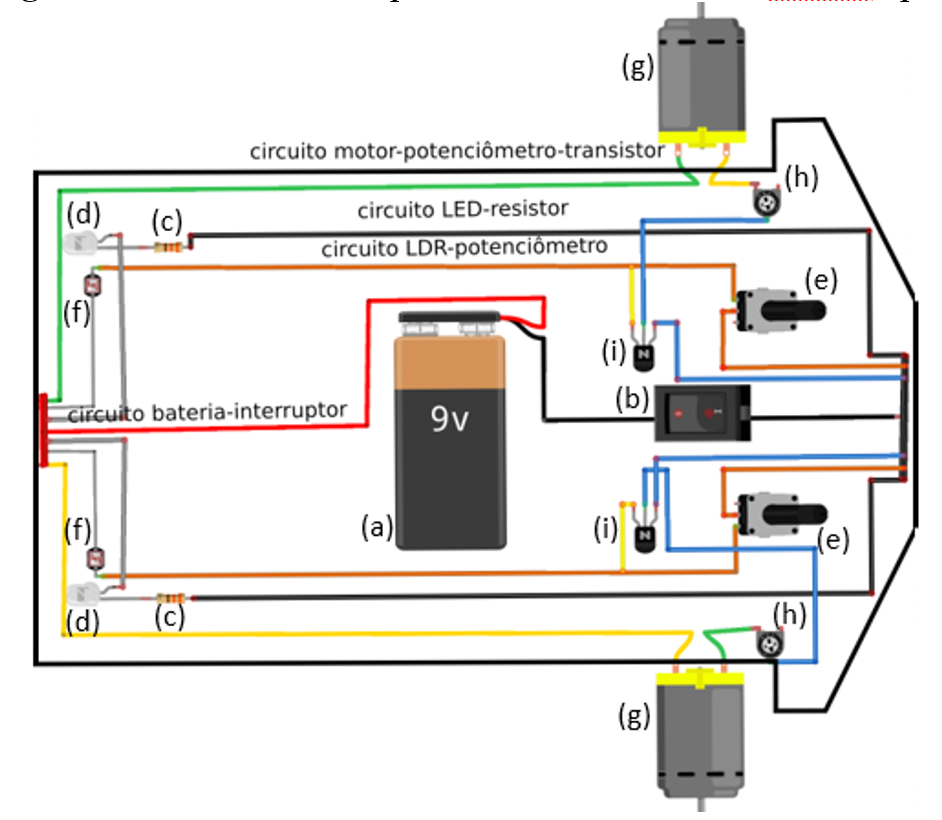
\includegraphics[width=\textwidth]{figuras/figura 2.png}
 \caption{Circuitos AGV para transistores NPN ou Mosfet tipo N:}
 \label{figura02}
 \source{Alves \citeyear[p. 51]{AlvesMonica2022}.}
\end{minipage}
\end{figure}

O funcionamento do robô é controlado por meio de quatro circuitos, espelhados a partir do circuito bateria-interruptor, \Cref{figura02}, sendo esse o primeiro circuito. O segundo é o circuito LED-resistor. O terceiro é o circuito LDR-potenciômetro, em que LED significa Light-emitting diode (Diodo emissor de Luz) e LDR Light Dependent Resistor (Resistor dependente de Luz). O quarto é o circuito motor-potenciômetro-transistor. Abstração que \textcite{AlvesMonica2022} explica da seguinte forma:

\begin{quote}
O primeiro composto pela fonte de alimentação (a), as estações negativa e positiva, e a chave liga/desliga (b), o segundo pelas estações negativa e positiva, pelo resistor (c) e o LED (d); o terceiro pelas estações negativa e positiva, pelo potenciômetro (e) e o LDR (f); e o quarto pelas estações negativa e positiva, pelo motor DC (g), o potenciômetro (h) e o transistor (i), \cite[p. 51]{AlvesMonica2022}.
\end{quote}

A investigação contou com a participação de uma professora da rede de ensino básico e uma discente de um curso de graduação em Matemática – Licenciatura. A produção dos dados foi feita por meio de registros escritos, vídeos, entrevistas e conversas intencionais com os participantes. Com efeito, a adoção de uma investigação exploratória partiu da necessidade de obtenção de materiais livres, sucatas, para a montagem do objeto/robô. Essa etapa inicial da exploração é fundamental, uma vez que é preciso entender, inicialmente, a funcionalidade e aplicação de cada componente, para então buscar objetos que possam conter os itens basilares para essa construção.

A partir dos dados obtidos na pesquisa exploratória, procedeu-se uma análise, com o objetivo de validar os dados e iniciar um processo de simulação. De acordo com \textcite[p. 4]{Vicente2005}, quando se tem dados empíricos, mas não um modelo, “[...] deverá ser criado um modelo inicial a ser aprimorado através de sucessivos testes". O modelo virtual do AVG foi criado no software Tinkercad, \Cref{figura03}. Vale ressaltar que o estudo de teorias matemáticas é essencial no processo demonstrado por este artigo, inclusas aqui as equações e inequações. Por meio delas, portanto, é possível determinar as características dos componentes que podem ser associados de forma que o robô tenha um funcionamento adequado.

\begin{figure}[htbp]
\centering
\begin{minipage}{0.95\textwidth}
 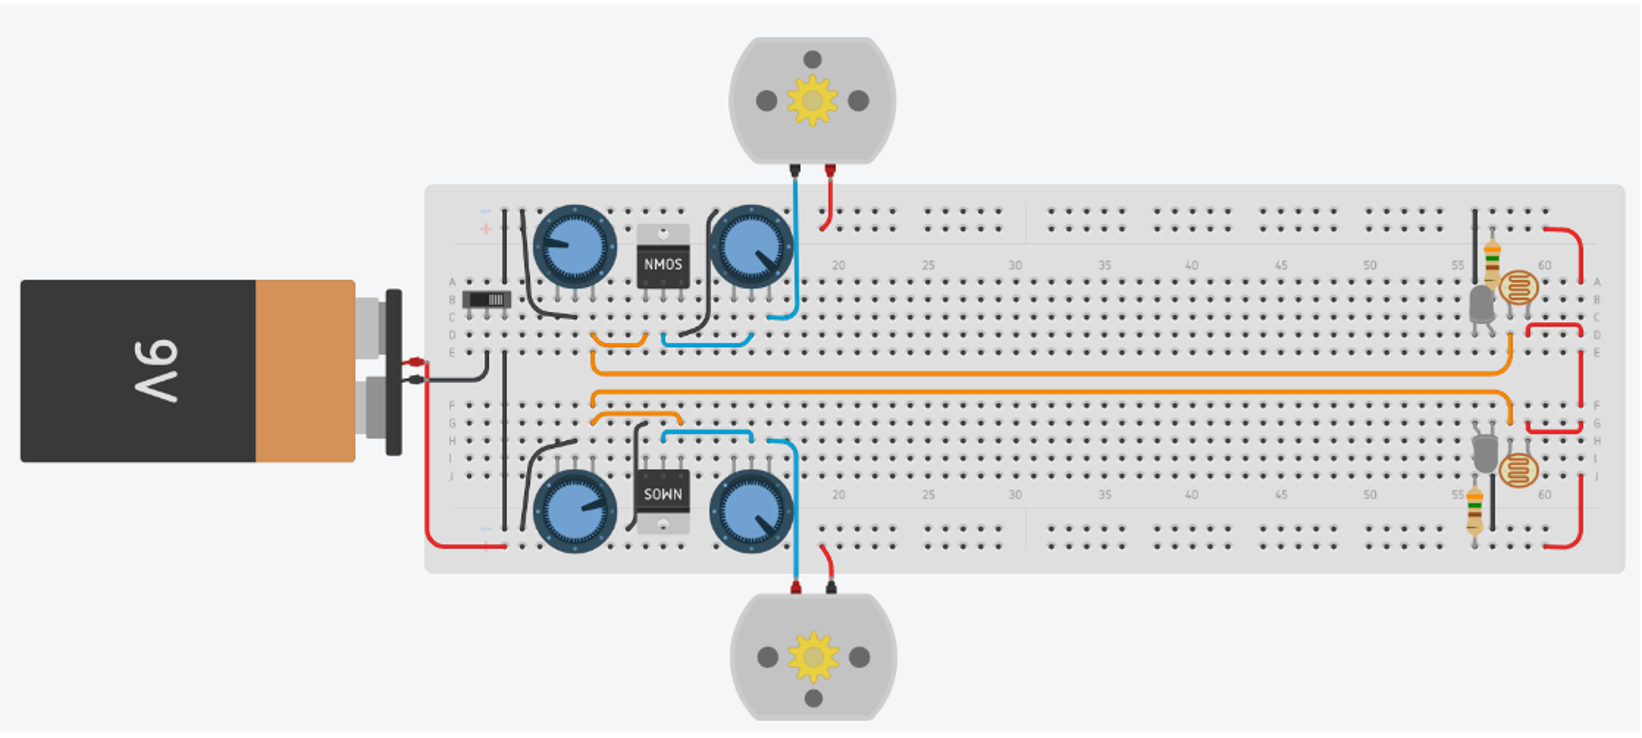
\includegraphics[width=\textwidth]{figuras/figura 3.png}
 \caption{Circuito no Tinkercard com transistor unipolar com terminais Gate, Drain e Source:}
 \label{figura03}
 \source{Alves \citeyear[p. 54]{AlvesMonica2022}.}
\end{minipage}
\end{figure}

Os resultados foram observados e analisados à luz das referências teóricas que oportunizam compreender a relevância da exploração, da descrição da construção de um objeto no ensino e da aprendizagem de tecnologias e da matemática, bem como da simulação. A observação e a análise possibilitaram a correção dos erros que foram gerados na construção do AGV, bem como perceber delineamentos para utilização do robô como um Micromundo de aprendizagem matemática.

\section{Desenvolvimento e análise dos resultados}\label{sec-organizacao}
Conforme preconiza \textcite[p. 267]{brasil2017}, o estudante deve desenvolver a competência de “[...] utilizar processos e ferramentas matemáticas, inclusive tecnologias digitais disponíveis para modelar e resolver problemas cotidianos, sociais e de outras áreas de conhecimento, validando estratégias e resultados”. Para alcançar tais resultados, faz-se necessário que o indivíduo assuma protagonismo no processo de ensino e aprendizagem, de forma que

\begin{quote}
[...] será necessário oportunizar situações em que os alunos participem cada vez mais intensamente na resolução das atividades e no processo de elaboração pessoal, em vez de se limitar a copiar e reproduzir automaticamente as instruções ou explicações dos professores. Por isso, hoje o aluno é convidado a buscar, descobrir, construir, criticar, comparar, dialogar, analisar, vivenciar o próprio processo de construção do conhecimento. \cite[p. 119]{Zabala1998}.
\end{quote}

Uma abordagem que propicia esse protagonismo é o ensino por investigação que “[...] não está diretamente associado a uma estratégia metodológica específica de ensino, mas configura-se como formas de agir e interagir que o professor utiliza em sala de aula” \cite[p. 3]{Snef2015}. É importante enfatizar que desenvolver habilidades para investigar é uma das metas que deveriam ser estabelecidas para a escola. Na perspectiva de \textcite[p. 2]{Ponte2003}.

\begin{quote}
[...] “Investigar” não é mais do que procurar conhecer, procurar compreender, procurar encontrar soluções para os problemas com que nos deparamos. Trata-se de uma capacidade de primeira importância para todos os cidadãos e que deveria permear todo o trabalho da escola, tanto dos professores como dos alunos.
\end{quote}

A proposta sobre a qual são feitas reflexões nesse trabalho, adotar o AGV como Micromundo de aprendizagem matemática pressupõe que o professor estimule a investigação, pois, para \textcite[p. 5]{BraumannCarlos2002}, “[...] aprender Matemática não é simplesmente compreender a Matemática já feita, mas ser capaz de fazer investigação de natureza matemática (ao nível adequado a cada grau de ensino)”. A referida proposta foi idealizada a partir de três elementos. Os dois primeiros: a bricolagem e a simulação de modelos digitais são duas concepções que, a princípio, parecem divergentes, mas que se complementam na perspectiva do terceiro elemento: a Inteligência Criadora, defendida por \textcite{Marina2009}.

Para proceder à análise da proposta, pretende-se partir da vivência de duas colaboradoras que desenvolveram suas experiências sob duas óticas distintas, uma sendo professora e outra estudante. A professora colaboradora, \textcite{AlvesMonica2022}, vivenciou a experiência desde a busca dos componentes eletrônicos e outros materiais para a construção do AGV, até o desenvolvimento de atividades para o processo de ensino e aprendizagem da Matemática. A estudante recebeu os materiais já retirados de sucatas, se concentrando na construção do AGV e na melhor forma de compartilhar os saberes oportunizados nesse processo.

De acordo com \textcite[p. 32]{Nunes2014}, “[...] a bricolagem em termos de investigação deve ser entendida como criação. Criação de um processo marcado pela experimentação, pelo uso/desuso de procedimentos, pelos achados e descartes de referências, de objetos de estudo, de perguntas e objetivos”. O processo de experimentação, a partir de materiais reaproveitados, estimula a criatividade e a curiosidade. Contudo, é igualmente marcado por alguns obstáculos próprios, provocados pela escolha da proveniência do material utilizado.

A primeira tarefa é providenciar as sucatas de onde podem ser retirados componentes eletrônicos úteis para a construção do dispositivo. Como \textcite[p. 32]{Nunes2014} enfatiza, “[...] o \emph{bricoleur} metodológico, bem como o \emph{bricoleur} de fim de semana, deve estar munido de um espírito construtor, catador de matérias e materiais que serão moldados, combinados e forjados com suas ferramentas, conforme sua intenção e necessidade”. \textcite{AlvesMonica2022} classificou a busca e coleta dos materiais como fácil, inclusive relatou a satisfação que os doadores desses materiais demonstraram em contribuir com a pesquisa. Vale ressaltar que é uma oportunidade de trabalhar a socialização de crianças e adolescentes, pois “[...] é na escola que se constrói parte da identidade de ser e pertencer ao mundo” \cite[p. 2]{BorsaJuliane2007}.

Se o construtor encontra dificuldades com o recolhimento e reutilização de objetos descartados, a aquisição dos componentes é uma opção. Este direcionamento limita as possibilidades de experimentação, mas ainda oportuniza o desenvolvimento da atividade a baixo custo, bem como a construção de conhecimentos. \textcite{Guimaraes2020} apresentam opções que podem facilitar o processo de aquisição dos materiais para a construção de um AGV. Pensando que se o acesso a sucatas é facilitado, o referido artigo pode ser usado como um guia, temos também uma outra face, ou seja, o acesso a uma diversidade de componentes, propiciando momentos enriquecedores de aprendizagem e estimula a criação.

Em seguida, deve ser feita a retirada dos componentes necessários, bem como daqueles que poderão ser utilizados em projetos futuros. Um ponto de preocupação é o descarte correto dos materiais não utilizados, pois a consciência ambiental deve ser também estimulada em processos de ensino e aprendizagem. O material a ser descartado pode ser doado para a reciclagem ou deixado em outros postos de coleta. A etapa exige cuidados, tanto com a segurança do construtor, exigindo o uso de equipamentos de proteção individual, quanto com a integridade dos componentes. \textcite[p. 43-44]{AlvesMonica2022} conta que “[...] não consegui realizar a extração de forma adequada e o calor excessivo danificou parcialmente o LDR. A danificação só foi constatada no momento de ligação do robô, que apresentou falhas sistemáticas”. Ao relatar “calor excessivo”, a autora informa que o calor excessivo do ferro de solda, somado à demora em retirar o componente, o danificou parcialmente.

Na etapa de construção da estrutura do AGV, as colaboradoras não encontraram dificuldades. Em sequência e por fim, os circuitos eletrônicos devem ser construídos. É nesta etapa que a bricolagem se intensifica. Na busca por conhecimentos, as colaboradoras buscaram referências sobre eletrônica e conteúdos matemáticos que poderiam ser explorados. Consequentemente, puderam desenvolver estratégias de montagem do dispositivo e de compatibilização dos modelos virtual e físico, entre outras coisas.

Na experiência vivenciada por \textcite[p. 47]{AlvesMonica2022}, “[...] na maior escala de dificuldade inclui-se a construção dos circuitos do robô. Esse momento exigiu diversos conhecimentos na área de Matemática e Física e a aplicação desses conhecimentos em uma atividade prática que se demonstrou complexa”. A autora ainda relata a necessidade de refazer os circuitos ao longo do processo. Por exemplo,

\begin{quote}
[...] o motor DC retirado do DVD de computador rotaciona de acordo com a polaridade da bateria (fonte de alimentação). Então, é necessário observar qual direção de rotação se deseja nas rodas do robô pra fazer a ligação na fonte. Na montagem as ligações tiveram que ser refeitas para obter a direção desejada, uma vez que esse fato não foi considerado inicialmente. \cite[p. 47]{AlvesMonica2022}.
\end{quote}

Além disso, os transistores, potenciômetros e resistores encontrados eram diferentes dos apresentados por \textcite{Guimaraes2020}, o que demandou esforço para as adaptações necessárias. Como afirma \textcite[p. 33]{Nunes2014}, a

\begin{quote}
[...] negociação pode ser pensada como um aspecto chave dentro do contexto da bricolagem, pois apresenta a necessidade de um pesquisador que se mantenha aberto, flexível e perceba que, em certos momentos, suas iniciativas de pesquisa devem ser repensadas, revistas, adaptadas.
\end{quote}

Para a discente colaboradora, que denominaremos Aprendiz, a fase inicial do processo foi um pouco trabalhosa devido à falta de conhecimentos sobre eletrônica. Nesse sentido, foram realizadas pesquisas para o desenvolvimento das habilidades necessárias. Segundo ela "\emph{[...] no começo, quando você olha uma imagem do circuito todo aí a gente fica meio perdido. Nossa, que que tem a ver? [...] mas conforme você vai separando, vai montando circuito por circuito, você vai entendendo pra que serve cada coisa}".

Terminada a fase de construção do AGV, as colaboradoras perceberam a necessidade de fazer testagens por partes, pois, se a testagem for feita somente ao final e o AGV apresentar alguma falha, é grande a dificuldade para encontrar o problema. Nenhum dos protótipos físicos construídos pelas colaboradoras funcionou após o término da construção. A busca pelos fatores que estavam desencadeando os problemas exigiu tempo e dedicação. Segundo a Aprendiz “\emph{[...] você vai montando seguindo o artigo, aí chega no final o que você espera é que você coloque a bateria e ele funcione. Só que aí, na hora que coloca e vê que não deu certo, isso assusta um pouco porque tem milhares de possibilidades de erros, e aí?}”

O processo de busca não é tão simples e, segundo a Aprendiz, contribuiu para seu crescimento pessoal no que tange à paciência. Em suas palavras, \emph{“[...] então, eu tinha que ter paciência de ver, de refazer, de olhar no circuito se eu estava montando alguma coisa errada e não desisti, até achar que o problema estava na bateria e depois que o problema estava no motor”}. Nesse sentido, alternativas para facilitar o processo foram exploradas, entre elas a simulação de modelos digitais, pois “[...] o conhecimento adquire uma nova dinâmica, passa a se realizar através de simulações, típico da cultura informatizada. Esse fato faz com que o computador seja também visto como um recurso didático a cada dia mais indispensável” \cite[p. 70]{BornattoGilmar2022}.

\textcite[p. 74]{Levy1993} afirma que “contrariamente à teoria, que tem como função primária explicar ou esclarecer um fenômeno, a simulação de modelos digitais seria antes operacional; provisional, ou mesmo normativa. Ela responde melhor à pergunta ‘como?’ do que a pergunta ‘por quê?’”. Contudo, o autor ressalta que além dos ganhos de tempo e benefícios de custo há um benefício cognitivo, pois a

\begin{quote}
[...] manipulação dos parâmetros e a simulação de todas as circunstâncias possíveis dão ao usuário do programa uma espécie de intuição sobre as relações de causa e efeito presentes no modelo. Ele adquire um conhecimento por simulação do sistema modelado, que não se assemelha nem a um conhecimento teórico, nem a uma experiência prática, nem ao acúmulo de uma tradição oral. \cite[p. 75]{Levy1993}.
\end{quote}

É nesta perspectiva que, o desenvolvimento do robô em um simulador oferece uma possibilidade de aprendizagem e exploração sem gerar perdas de materiais. A partir da prática, da experiência de testar, errar e perder material, optou-se por realizar simulações no software Tinkercad. Isso porque “[...] essa ferramenta [...] facilitou o entendimento das ligações dos componentes, a simulação dos LEDs e a visualização do circuito como um todo” \cite[p. 47-48]{AlvesMonica2022}. Consequentemente, a partir das vivências dessa autora e da Aprendiz, pode-se constatar a contribuição da simulação para a aprendizagem dos envolvidos. Essa experiência foi reproduzida no desenvolvimento de uma disciplina do ensino superior, na qual a construção do AGV foi trabalhada. A percepção dos discentes corroborou esse direcionamento, o que pode ser percebido na fala de um deles, obtidas em uma das atividades do curso:

\begin{quote}
\emph{[...] minha primeira impressão ao assistir o vídeo do AGV funcionando foi de que o funcionamento dos seus circuitos seria complicado e inacessível para pessoas sem conhecimento aprofundado. Foi uma surpresa ver [ao utilizar o Tinkercad] que, além de não ser complexo, ele consiste em poucas peças e pode ser construído por praticamente qualquer pessoa} (APRENDIZ em Entrevista).
\end{quote}

A experiência de utilizar simulador nessa disciplina permitiu aos estudantes fazerem testes com um quarto circuito transistor-potenciômetro-motor mais simples, com apenas transistor-motor. Outro ponto foi o de repensar a estrutura dos componentes sem placas de apoio, mas simplesmente soldados por fio e fixados com cola quente na estrutura do AGV, facilitando a produção do mesmo.

É importante ressaltar que a simulação tem limitações. De acordo com \textcite[p. 2]{BritoAntonio2001}, “[...] tal processo introduz, só por si, uma fonte de incertezas nos resultados que daí se retirem, uma vez que o modelo será sempre uma “aproximação” ao sistema real e não o verdadeiro sistema”. \textcite{AlvesMonica2022} relata que o protótipo virtual do AGV, construído por ela, funcionou perfeitamente, entretanto o protótipo físico não. Portanto, fica claro que só a construção do protótipo físico pode não conduzir ao êxito e só a simulação também não. Daí surgiu a necessidade de compatibilização dos dois protótipos. Segundo \textcite[p. 80]{Gravinha1999} “[...] os ambientes com recursos de modelagem e simulação também possibilitam tratar a Matemática como ferramenta para resolução de problemas em outras áreas do conhecimento”.

Partindo dos fatos observados, foi estruturada uma linha de ação que tornou possível transpor os obstáculos ao desenvolvimento do projeto, com o auxílio de ferramentas matemáticas. A seguir será apresentado como essas ferramentas foram utilizadas por \textcite{AlvesMonica2022} para a correção dos erros e do funcionamento do AGV.

Na \Cref{figura04}, temos a visão do robô de forma frontal e cada região representa uma das citações possíveis para o funcionamento ou não do AVG, a região A é quando o sensor do circuito da roda esquerda reconhece a linha preta. Na região B nenhum dos sensores reconhecem a linha preta. Na região C o sensor do circuito da roda direita reconhece a linha preta.

\begin{figure}[htbp]
\centering
\begin{minipage}{0.99\textwidth}
 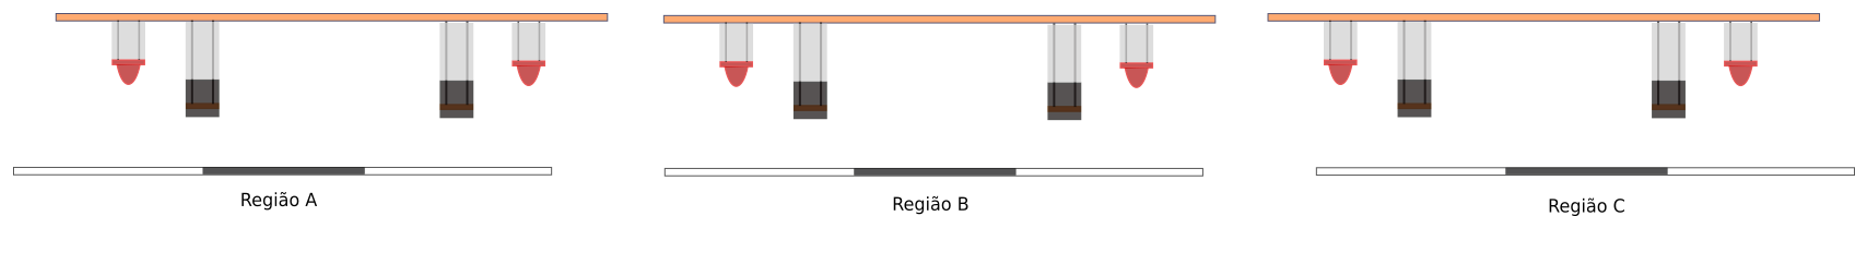
\includegraphics[width=\textwidth]{figuras/figura 4.png}
 \caption{AGV:}
 \label{figura04}
 \source{Acervodos autores.}
\end{minipage}
\end{figure}

Vejam que se o LDR fica sobre a linha preta, envia uma corrente elétrica menor para o transistor. Isso ocorre devido ao fato da cor preta absorver quase toda a luz incidente sobre ela, não permitindo a reflexão da luz do LED no fotoresistor LDR. Consequentemente, com a corrente menor para o transistor, ela que chega ao conjunto potenciômetro/motor diminui, provocando a desaceleração ou repouso da roda.

Já na construção do modelo real, realizada pela autora, o circuito da roda esquerda do AGV funcionava normalmente e o da direita não, o que motivou a realização de testes de leitura dos LDRs. Dessa forma, obteve-se os seguintes dados:

%inicio
% Please add the following required packages to your document preamble:
% \usepackage{graphicx}
% \usepackage[table,xcdraw]{xcolor}
% If you use beamer only pass "xcolor=table" option, i.e. \documentclass[xcolor=table]{beamer}
\begin{table}[htpb]
\caption{Faixa de leitura dos LDRs.}
\label{tabela1}
\centering
\begin{tabular}{c c c}
\hline
\multicolumn{3}{c}{\cellcolor[HTML]{CFE7F5} \textbf{AVG terceira}}                         \\ \hline
\rowcolor[HTML]{CFE7F5} 
\textbf{LOCAL} & \multicolumn{1}{|c|}{\cellcolor[HTML]{CFE7F5} \textbf{Circuíto - roda esquerda}} & \multicolumn{1}{c}{\cellcolor[HTML]{CFE7F5} \textbf{Circuíto - roda direita}} \\ \hline
\cellcolor[HTML]{CFE7F5} \textbf{Região A} & \multicolumn{1}{|c|}{5.000  $K\Omega$} & 18.500 $K\Omega$ \\ \hline
\cellcolor[HTML]{CFE7F5} \textbf{Região B} & \multicolumn{1}{|c|}{4.000 $K\Omega$} & 18.400 $K\Omega$ \\ \hline
\cellcolor[HTML]{CFE7F5} \textbf{Região C} & \multicolumn{1}{|c|}{4.000 $K\Omega$} & 20.000 $K\Omega$ \\ \hline
\end{tabular}%
\source{Acervo dos autores.}
\end{table}
%fim

Note que as faixas de variação são muito díspares, apesar da estrutura e circuitos serem similares, de onde concluiu-se que o potenciômetro da roda direita perdeu parte de sua funcionalidade. Recordando a causa do defeito no componente se deve a forma como ele foi obtido, já supracitado. Constata-se aqui a importância do modelo virtual, pois nele é possível criar, simular e validar o circuito em seu funcionamento. Se fosse feito todo no real, haveria possibilidade de erros e perdas de material. Simular virtualmente poupa perda de material físico e testa as combinações para que se tenha a construção do circuito mais eficiente. Em projetos de grande magnitude, o virtual é uma economia significativa. Mesmo com projeto no virtual funcionando, existe a mínima chance de o projeto no real não funcionar, mas aí é fruto de algum componente, como aconteceu no protótipo do AGV, cujo componente potenciômetro estava apresentando leituras inconsistentes.

Os transistores utilizados em \textcite{AlvesMonica2022} foram unipolares. Esses transistores controlam a corrente do terminal \emph{Drain} para o \emph{Source}, a partir da tensão do Gate para o \emph{Source}, como pode ser interpretado no gráfico da \Cref{figura05}.

\begin{figure}[h!]
\centering
\begin{minipage}{0.7\textwidth}
 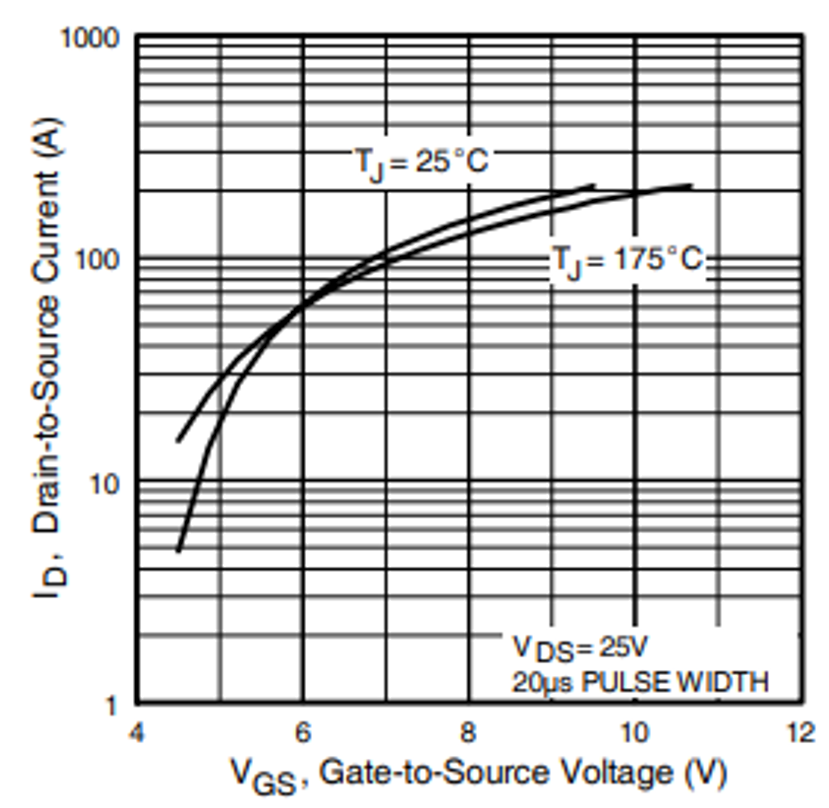
\includegraphics[width=\textwidth]{figuras/figura 5.png}
 \caption{Gráfico de características de transferências típicas do transistor mosfet IRFZ48N:}
 \label{figura05}
 \source{\textcite[p. 3]{infineon2010}.}
\end{minipage}
\end{figure}

Observe no gráfico de características de transferências típicas que, há uma temperatura de junção de 25ºC - temperatura aproximada que se trabalha no AGV - quando a tensão \emph{Gate-to-Source}, $V_{GS}$, é menor que $4,5V$, a corrente \emph{Drain-to-Source}, ¨$I_D$, é nula.

Além disso, de acordo com \textcite[p. 63-65]{AlvesMonica2022}, como há um material de alta resistência entre o \emph{Gate} e os outros terminais, a corrente que circula pelo Gate é próxima de zero, podendo ser, neste caso, considerada nula. Sendo assim, a tensão \emph{Gate-to-Source} será a tensão do divisor de tensão no circuito LDR-potenciômetro, a saber:

$$V_{POT} = \frac{V_{FA}}{R_{LDR}+R_{POT}}R_{POT}$$

Ou seja, $V_{GS} = V_{POT}$, em que ele é a tensão do divisor e também a diferencial de tensão no potenciômetro (em volts), (em volts), $V_{FA} = 9V$ é a tensão da fonte de alimentação, $R_{LDR}$ é a resistência do LDR (em $\Omega$) e $R_{POT}$ é a resistência do potenciômetro do circuito LDR-potenciômetro (em $\Omega$), que precisa ser calculada considerando as condições necessárias para a movimentação do AGV.

Portanto, em $V_{GS} < 4,5V$ a corrente $I_D$ é nula e o motor fica em repouso. Se $V_{GS} > 4,5V$, existe corrente que pode fazer com que o motor entre em funcionamento. Vale ressaltar que, no caso do motor utilizado em \textcite{AlvesMonica2022}, as informações contidas no datasheet indicam que ele funcionará com correntes acima de $0,08A$ e, caso contrário, estará em repouso.

Quando o LDR esquerdo está acima da linha preta, conforme a Tabela \ref{tabela1}, a resistência do LDR $é R_{LDR} \approx 5000\Omega$ e o motor deverá estar em repouso, ou seja, $V_{GS} < 4,5V$. Daí

$$4,5 > \frac{9}{5000 + V_{POT}}V_{POT} \iff R_{POT} < 5000 \Omega$$

Nas outras regiões, a resistência do LDR, de acordo com a \Cref{tabela1}, é $R_{LDR} \approx 4000\Omega$ e o motor deverá estar em movimento, ou seja, $V_{GS} > 4,5V$. Daí

$$4,5 < \frac{9}{4000 + V_{POT}}V_{POT} \iff R_{POT} > 4000 \Omega$$

Quando o LDR direito está acima da linha preta, a resistência do LDR, segundo a \Cref{tabela1}, é $R_{LDR} \approx 20000\Omega$ e o motor deverá estar em repouso, ou seja, $V_{GS} < 4,5V$. Daí

$$4,5 > \frac{9}{20000 + V_{POT}}V_{POT} \iff R_{POT} < 20000 \Omega$$

Nas outras regiões, a resistência do LDR, de acordo com a \Cref{tabela1}, será, $R_{LDR} \approx 18400\Omega$ e o motor deverá estar em movimento, ou seja, $V_{GS}  > 4,5V$. Daí

$$4,5 < \frac{9}{18400 + V_{POT}}V_{POT} \iff R_{POT} > 18400 \Omega$$

A princípio, foram utilizados potenciômetros de $20.000\Omega$ para ambos os circuitos, contudo a roda direita não obteve o funcionamento desejado, funcionando com o LDR sobre a linha preta com qualquer regulagem do potenciômetro do circuito LDR-potenciômetro. Foi feita, portanto, a testagem do potenciômetro com o multímetro, atingindo a faixa de $30\Omega$ a $18.000\Omega$.  Por conseguinte, concluiu-se que essa escolha não foi adequada, pois potenciômetros podem ter perda de eficiência e não atingir as faixas previstas. Assim, o potenciômetro foi substituído por um de $50.000\Omega$ fazendo, enfim, com que o AGV funcionasse.


\section{Considerações finais}\label{sec-conclusao}
A experiência física mostrou que as altas temperaturas do ferro de solda, usado na retirada de componentes eletrônicos e favorecido com a demora na retirada dos componentes, geraram perdas na eficiência dos mesmos. As ferramentas matemáticas se tornaram indispensáveis para a correção de parâmetros essenciais para o funcionamento do robô, sem perdas de materiais e tempo, sem a necessidade de (des)montar circuitos para testagens ao acaso e corrigindo os problemas gerados por um fator inesperado. Ademais, o estudo realizado a partir de circuitos unipolares e bipolares evidenciou a possibilidade de produzir robôs com circuitos distintos para cada uma das rodas, o que, segundo \textcite[p. 50]{AlvesMonica2022}, é “[...] adequado para uma proposta de utilizar sucatas e diferentes componentes que são aproveitados”. De acordo com a autora, essa percepção foi construída mostrando como a Matemática pode contribuir para produzir circuitos mais eficientes e diversificados.

O trabalho com robótica educacional perpassa por um processo de exploração e investigação, principalmente quando trabalhamos com materiais livres, sucatas eletrônicas. Nesse processo enriquecedor, percebemos e aprendemos que o simulador virtual é fundamental no processo de construção de um dispositivo real. A simulação permite visualizar e testar os recursos sem gerar danos aos materiais físicos, mas sem a Matemática, sem a interpretação dos dados produzidos na simulação, os problemas gerados a partir das combinações/simulações não serão resolvidos.

É comum observarmos, em pesquisas de Robótica Educacional, trabalhos que apresentem soluções para problemas através do método de tentativa e erro. Conclui-se, a partir desta investigação, que a utilização desse método com materiais livres na RE é custosa e atrasa o processo, além de ir contra o objetivo de ensinar sobre preservação do meio ambiente e sustentabilidade através da reutilização de sucatas tecnológicas.

A experiência com a construção do AGV é mais que a construção de um robô, é a afirmação da importância da Matemática, do simulador virtual na concepção do real, do tangível que ainda irá passar por um processo de teste. O real e virtual se comunicam para resolver os problemas, mas a Matemática apresenta os caminhos da solução. São três elementos inseparáveis para um sucesso em menor tempo, menos prejuízos ou perdas. Qualquer decisão contrária será um caminho mais longo e tortuoso, sem esquecer que fere um princípio da robótica livre de não gerar uma educação tecnológica sustentável.

Alguns desses testes já iniciados motivaram os autores desse trabalho a propor circuitos mais eficientes para seguir a linha, sem muitas dificuldades no controle do mesmo, porém com perdas na velocidade. Nessas alterações de circuitos, os resultados matemáticos apresentados neste artigo continuam valendo, talvez necessitando somente de pequenos ajustes. São duas as alterações nos circuitos no quarto circuito motor-potenciômetro-transistor: a retirada do potenciômetro e a ligação do motor a partir do \emph{Source} (respectivamente, Emissor) do transistor unipolar canal N (respectivamente, bipolar NPN), conforme ilustrada pela \Cref{figura06}. Nesse caso, o \emph{Drain} (respectivamente, Coletor) é ligado no terminal positivo, e um dos terminais do motor ligado no \emph{Source} (respectivamente, Emissor) e o outro no terminal negativo.

\begin{figure}[htbp]
\centering
\begin{minipage}{0.99\textwidth}
 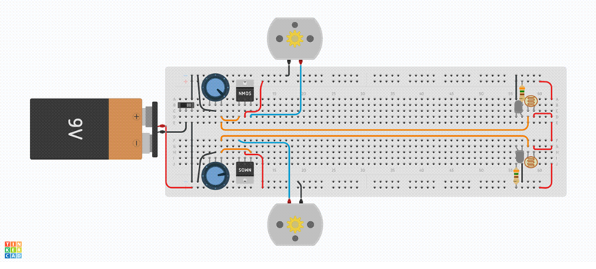
\includegraphics[width=\textwidth]{figuras/figura 6.png}
 \caption{Circuito no Tinkercard para unipor canal N com terminais \emph{Gate, Drain e Source}:}
 \label{figura06}
 \source{Acervo dos autores.}
\end{minipage}
\end{figure}

A alteração do posicionamento do motor no circuito motor-transistor gera perdas de tensão e assim ganho de precisão. Como podemos ver em \textcite{Maganha2023} para transistores bipolares NPN, quando o motor está ligado a partir do Emissor, ele obtém uma tensão menor que a mínima da tensão do Coletor-Emissor e da tensão Base-Emissor. Importante salientar que a tensão do Coletor-Emissor é \textbf{igual} à soma das tensões Coletor-Base e Base-Emissor. Como há grande resistência no LDR-potenciômetro, a tensão no motor será menor do que a tensão Base-Emissor. Diferentemente do caso de ligar o motor ao coletor e na estação positiva, no qual ele obtém a tensão Coletor-Emissor, próxima de 9V, tornando-os mais velozes e assim, mais impreciso. É desnecessário utilizar o potenciômetro (h) na \Cref{figura02} no circuito motor-transistor neste tipo de proposta.

Outro ponto explorado foi as diferentes maneiras de posicionar e soldar os componentes nos circuitos, em que os circuitos mais fáceis de serem produzidos são aqueles realizados sem a placa de circuito, utilizando somente fios, soldas e cola quente para fixar os componentes. Já os circuitos mistos com tipos diferentes de transistores e potenciômetros para cada roda, produzem carrinhos com a mesma eficiência.

\printbibliography\label{sec-bib}

% if the text is not in Portuguese, it might be necessary to use the code below instead to print the correct ABNT abbreviations [s.n.], [s.l.]
%\begin{portuguese}
%\printbibliography[title={Bibliography}]
%\end{portuguese}

%full list: conceptualization,datacuration,formalanalysis,funding,investigation,methodology,projadm,resources,software,supervision,validation,visualization,writing,review
\begin{contributors}[sec-contributors]
    \authorcontribution{Fernando Barbosa}[conceptualization, formalanalysis,  investigation, methodology, projadm, resources, supervision, visualization, writing, review]
    \authorcontribution{Daniel Guimarães}[conceptualization, datacuration, formalanalysis,  funding,  investigation, methodology, projadm, resources, software, validation, visualization, writing, review]
    \authorcontribution{Élida Silva}[conceptualization, formalanalysis,  methodology, projadm, resources, software, supervision, visualization, writing, review]
    \authorcontribution{Deive Alves}[conceptualization, formalanalysis, methodology, software, writing, review]
    \authorcontribution{Mônica Alves}[datacuration, investigation, writing]
\end{contributors}

\end{document}

